برای طراحی یک شبکه عصبی که تساوی دو ورودی باینری x و y را خروجی دهد از
\lr{XNOR} 
استفاده می‌کنیم.
می‌توانیم از دو لایه مخفی استفاده کنیم. در این حالت، ابتدا می‌توانیم ورودی‌ها را به دو گیت
\lr{AND}
و
\lr{NOR}
فرستاده و سپس خروجی این دو گیت را به یک گیت 
\lr{OR}
متصل کنیم. شبکه به شکل زیر خواهد بود:

\begin{center}
	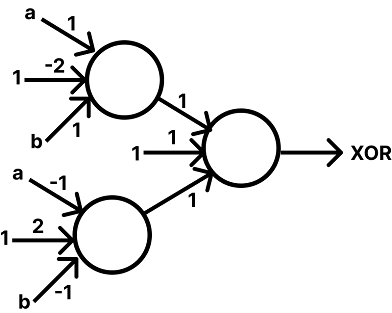
\includegraphics{pic}
\end{center}

این شبکه عصبی یک گیت
\lr{XNOR}
را شبیه‌سازی می‌کند. وقتی
\lr{x}
و
\lr{y}
هر دو 1 یا هر دو 0 باشند، خروجی شبکه بیش از
\lr{threshold}
(مثلا
\lr{0.5}
 ) خواهد بود.

اما برای تشخیص تساوی برای هر ترکیبی از دو عدد صحیح، مسئله بسیار پیچیده‌تر است. برای تشخیص تساوی دو عدد صحیح، ممکن است باید از شبکه‌های عصبی عمیق‌تر با تعداد بیشتری از نورون‌ها استفاده کنیم و از روش‌های مختلفی برای تشخیص نتایج استفاده کنیم، مثلا باید عدد را به فرم باینری تبدیل کرده و سپس هر بیت را بررسی کنیم. برای این منظور باید از الگوریتم‌های یادگیری ماشین پیچیده‌تری استفاده کنیم و ممکن است نیاز به داده‌های آموزشی بیشتری داشته باشیم.